% Copyright 2026 Sreeram Anil
% SPDX-License-Identifier: CC-BY-4.0
% =============================================================================
%  Bar-delta pack filtering — pack-level (multi-cell) family
% =============================================================================
\chapter{Bar-Delta Pack Filtering (BarDelta)}
\label{ch:bardelta}

\section*{At a glance}
\begin{tabular}{@{}l>{\raggedright\arraybackslash}p{0.76\textwidth}@{}}
Family & pack-level (common state + per-cell deviation) \\
Header & \texttt{include/estkit/pack/bar\_delta.hpp}, \texttt{pack\_common.hpp} \\
Registered name & \texttt{BarDelta} \\
Estimated quantities & $\bar{\vx}=[\bar\soc,\bar v_1,\bar v_2,\bar h]^\T$ and $\{\Delta \soc_j,\Delta\rho_j,\Delta q_j\}_{j=1}^{N_c}$ \\
Filters per module & one $n_x=4$ EKF at $f_s$ + $N_c$ three-state KFs at $f_s/10$ \\
Cost per step & $\SI{542}{\nano\second}$ for $N_c=12$ cells (\SI{45}{\nano\second} per cell) \\
Memory & \SI{5616}{\byte} for the whole module \\
Bus load & $N_c=12$ numbers per sample (cell voltages to the module master) \\
Primary references & \cite{plett2009bardelta,plett2016bms2,plett2004ekf3} \\
\end{tabular}

\section{Motivation and aerospace/BMS relevance}
An eVTOL traction battery is a series--parallel assembly of several hundred cells. Certification
of the usable-energy and usable-power estimates \cite{rtca2017do311a,yang2021evtol} is written in
terms of the \emph{weakest} cell on discharge and the \emph{strongest} cell on charge, not in
terms of an average, so a pack BMS must produce a state of charge for \emph{every} cell, not one
number for the string. The obvious implementation --- one extended Kalman filter per cell, the
\estname{Decentralized-EKF} baseline of Chapter~\ref{ch:decentralizedekf} --- multiplies the
computational and memory cost of the cell-level estimator by the number of cells. On the
benchmark module of $N_c=12$ cells that is \SI{3.8}{\micro\second} and \SI{51}{\kibi\byte} per
sample; scaled to the $\sim$\num{400} cells of a flight battery it is \SI{130}{\micro\second} and
\SI{1.7}{\mebi\byte}, which no automotive-grade BMS microcontroller will provide, and it is
\emph{wasted} work: the twelve state trajectories are nearly identical.

They are nearly identical for a structural reason. Cells in series carry exactly the same
current. The fast dynamics of the equivalent-circuit model (Chapter~\ref{ch:ecm}) --- the two RC
branches with $\tau_1\approx\SI{5}{\second}$, $\tau_2\approx\SI{120}{\second}$, and the
hysteresis state --- are driven only by that shared current, so they are \emph{common} to all
cells up to the manufacturing spread of the parameters. Only the slow part differs: the initial
SOC imbalance and the divergence caused by capacity spread, both of which move on the time scale
of a whole mission.

Bar-delta filtering \cite{plett2009bardelta,plett2016bms2} is the exploitation of that structure.
One full nonlinear filter --- the \emph{bar} filter --- is run on a fictitious \emph{average
cell}, driven by the average of the measured cell voltages; and one very small filter per cell
--- the \emph{delta} filters --- tracks only the deviation of that cell from the average, at a
reduced update rate. The cost becomes $\mathcal{O}(n_x^3) + N_c\,\mathcal{O}(1)$ instead of
$N_c\,\mathcal{O}(n_x^3)$, i.e.\ essentially the cost of a \emph{single}-cell estimator plus a
per-cell term small enough to run on the cell-monitor slaves themselves.

The idea is the direct battery analogue of a very old one in navigation: estimate the large,
strongly observable common mode with a full filter and the small, weakly observable differential
modes with reduced-order filters. In that sense this chapter is the entry point to the
common-state formulation that Chapters~\ref{ch:infofusion}--\ref{ch:consensus} then re-derive as
an optimal-fusion problem.

\section{Problem statement and assumptions}
A module of $N_c$ cells in series carries the common current $i_k$ (discharge positive) and is
measured by $N_c$ voltage channels $v_{j,k}$, $j=1,\dots,N_c$, and $N_c$ temperature channels
$T_{j,k}$. Cell $j$ obeys the ESC model of Chapter~\ref{ch:ecm} with its own parameters:
\begin{align}
\soc_{j,k+1} &= \soc_{j,k} - \eta(i_k)\,\dt\,i_k/(3600\,Q_j), \label{eq:bd-cellz}\\
v_{j,k} &= \ocv(\soc_{j,k},T_{j,k}) + M h_{j,k} - v_{1,j,k} - v_{2,j,k} - R_{0,j}(T_{j,k})\,i_k + e_{j,k},
\label{eq:bd-cellv}
\end{align}
where $Q_j$ [\si{\ampere\hour}] is the total capacity of cell $j$, $R_{0,j}$ its series
resistance, $\eta$ the coulombic efficiency, $M$ the hysteresis magnitude and
$e_{j,k}\sim\N{0}{\sigma_v^2}$ the (independent) voltage-sensor noise of channel $j$.

Define the pack-average (\emph{bar}) quantities and the per-cell deviations (\emph{deltas})
\begin{equation}
\bar\soc_k = \frac{1}{N_c}\sum_{j} \soc_{j,k},\qquad
\Delta\soc_{j,k} = \soc_{j,k} - \bar\soc_k, \qquad \sum_j \Delta\soc_{j,k} = 0,
\label{eq:bd-decomp}
\end{equation}
and likewise $\bar v_1,\bar v_2,\bar h$. The method rests on three assumptions.

\begin{assumption}[Shared current]\label{as:bd-current}
All cells of the string carry the same current $i_k$. This is exact for a series string and
approximately true within a parallel group.
\end{assumption}
\begin{assumption}[Small deviations]\label{as:bd-small}
$|\Delta\soc_j|$ is small enough that a \emph{first-order} expansion of the overpotential terms
of \eqref{eq:bd-cellv} about the average cell is accurate. The benchmark spread is
$\sigma_{\Delta\soc}(0)=\SI{1.5}{\percent}$ (\SI{5}{\percent} in \texttt{large\_imbalance}); the
weak-cell scenario grows it to $\approx\SI{10}{\percent}$ over one mission.
\end{assumption}
\begin{assumption}[Slow deviations]\label{as:bd-slow}
The deviations change only through parameter differences, hence at a rate proportional to $|i|$
and to the relative parameter spread --- three orders of magnitude slower than the RC dynamics.
This is what allows the delta filters to run at a reduced rate.
\end{assumption}

\section{Derivation}

\paragraph{The bar filter.} Averaging \eqref{eq:bd-cellv} over $j$ gives
\begin{equation}
\bar v_k \;\triangleq\; \frac{1}{N_c}\sum_j v_{j,k}
 = \underbrace{\ocv(\bar\soc_k,\bar T_k) + M\bar h_k - \bar v_{1,k} - \bar v_{2,k} - \bar R_0 i_k}_{\displaystyle h(\bar{\vx}_k,\bar{\vu}_k)}
 \;+\; \underbrace{\tfrac12 \ocv''(\bar\soc_k)\,\overline{\Delta\soc^2}}_{\text{Jensen gap } J_k}
 \;+\; \bar e_k + \mathcal{O}(\Delta^3),
\label{eq:bd-baraverage}
\end{equation}
because the first-order terms cancel by $\sum_j\Delta\soc_j=0$ and by
$\sum_j (R_{0,j}-\bar R_0)=0$. Two consequences are used by the implementation.

\emph{(i)} $\bar e_k = N_c^{-1}\sum_j e_{j,k}$ has variance $\sigma_v^2/N_c$: averaging $N_c$
independent voltage channels buys a factor $N_c$ in measurement-noise power. The common-mode
error, however, does not average down, so the bar filter is given
\begin{equation}
\mR_{\text{bar}} = \frac{\sigma_v^2}{N_c} + \sigma_{\text{mdl}}^2 + \big(\bar R_0\sigma_i\big)^2,
\label{eq:bd-Rbar}
\end{equation}
with $\sigma_{\text{mdl}}$ the residual error of representing the module by one average cell and
$(\bar R_0 \sigma_i)^2$ the current-sensor term inherited from the cell model.

\emph{(ii)} $J_k$ is a genuine bias: the average of the cell voltages is \emph{not} the voltage
of the average cell, because $\ocv$ is curved. The implementation removes it explicitly using the
delta estimates,
\begin{equation}
\hat J_k = \frac{1}{N_c}\sum_j\Big[\ocv\big(\hat{\bar\soc}_k + \Delta\hat\soc_{j,k},\,\bar T_k\big) - \ocv\big(\hat{\bar\soc}_k,\bar T_k\big)\Big],
\label{eq:bd-jensen}
\end{equation}
and feeds $\bar v_k - \hat J_k$ to the bar filter. With the benchmark spread $\hat J$ reaches
\SI{6}{\milli\volt} in \texttt{large\_imbalance}, three times the sensor noise.

Everything else about the bar filter is the cell-level EKF of Chapter~\ref{ch:ekf} applied to the
nominal parameter set:
\begin{equation}
\bar{\vx}^-_k = f(\bar{\vx}^+_{k-1},\bar{\vu}_{k-1}),\quad
\Pminus_k = \mF\Pplus_{k-1}\mF^\T + \mQ, \quad
\bar{\vx}^+_k = \bar{\vx}^-_k + \mK_k\big(\bar v_k - \hat J_k - h(\bar{\vx}^-_k,\bar{\vu}_k)\big).
\label{eq:bd-barekf}
\end{equation}

\paragraph{The delta measurement.} Subtracting \eqref{eq:bd-baraverage} from
\eqref{eq:bd-cellv},
\begin{equation}
y_{\Delta,j,k} \;\triangleq\; v_{j,k} - \bar v_k
 = \underbrace{\ocv(\bar\soc_k + \Delta\soc_{j,k}) - \ocv(\bar\soc_k)}_{\text{SOC deviation}}
 - \underbrace{\Delta\rho_{j}\,w_k}_{\text{impedance deviation}}
 + \underbrace{M\,\Delta h_{j,k}}_{\text{hysteresis}} + \tilde e_{j,k},
\label{eq:bd-deltameas}
\end{equation}
where $w_k$ is the \emph{impedance regressor}. Two models of the impedance deviation are
implemented. With \texttt{include\_rc\_in\_regressor = false} (the default, and Plett's original
choice) $w_k = \bar R_0(\bar T_k)\,i_k$ and $\Delta\rho_j \bar R_0 = \Delta R_{0,j}$ is the
classical delta-resistance in ohms; with the option set, $w_k = \bar R_0 i_k + \bar v_1 + \bar
v_2$ is the \emph{total} overpotential of the average cell and $\Delta\rho_j$ is a dimensionless
\emph{relative} impedance deviation, which is exact when all impedances of a cell scale together
(area/porosity spread). The measurement noise of \eqref{eq:bd-deltameas} is
\begin{equation}
\Var{\tilde e_{j}} = \sigma_v^2\Big(1 - \tfrac1{N_c}\Big) + \big(\epsilon_R\,w^{\mathrm{tot}}_k\big)^2 + \sigma_h^2,
\label{eq:bd-Rdelta}
\end{equation}
the first term because $v_j$ and $\bar v$ share $1/N_c$ of the same noise, the second because the
impedance spread is not perfectly described by one scalar times one regressor (an aged cell
scales $R_0$ and $R_1$ but not $R_2$), the third for the hysteresis spread.

\paragraph{The delta dynamics: why a random walk is not enough.} Subtracting the coulomb-counting
equation \eqref{eq:bd-cellz} of cell $j$ from that of the average cell gives the deviation
dynamics \emph{exactly}:
\begin{equation}
\Delta\soc_{j,k+1} = \Delta\soc_{j,k} + a_k\,\Delta q_j ,\qquad
a_k = -\frac{\eta(i_k)\,i_k\,\dt_u}{3600\,Q_{\text{nom}}},\qquad
\Delta q_j = \Big(\frac{1}{Q_j} - \frac{1}{\bar Q}\Big)Q_{\text{nom}},
\label{eq:bd-deltadyn}
\end{equation}
with $\bar Q^{-1} = N_c^{-1}\sum_j Q_j^{-1}$ and $\dt_u$ the delta-filter update interval. The
deviations are therefore driven by the shared current through the unknown \emph{inverse-capacity
deviation} $\Delta q_j$ ($\Delta q_j > 0$ means cell $j$ is weaker than the average, and
$\sum_j\Delta q_j = 0$). Equation \eqref{eq:bd-deltadyn} is a \emph{ramp}, not a random walk: for
the benchmark weak cell ($\SI{12}{\percent}$ capacity loss, $\Delta q \approx 0.157$) the
deviation grows at $\SI{4e-5}{\per\second}$ in cruise and reaches $\num{0.10}$ over the
\SI{2010}{\second} mission. A scalar random-walk model of $\Delta\soc$ tracks a ramp only with a
lag $\approx v\,\dt_u(1-K)/K$; achieving a lag below \num{0.005} would require a process noise so
large that the estimate becomes noisy everywhere else. The delta filter therefore carries
$\Delta q_j$ as a third state (this is Plett's delta-capacity filter, folded into the same small
filter), and $\Delta\rho_j,\Delta q_j$ are modelled as slow random walks:
\begin{equation}
\bm{d}_j = \begin{bmatrix}\Delta\soc_j\\ \Delta\rho_j\\ \Delta q_j\end{bmatrix},\quad
\mA_k = \begin{bmatrix}1&0&a_k\\0&1&0\\0&0&1\end{bmatrix},\quad
\mQ_\Delta = \diag\big(\sigma_{\Delta\soc}^2\dt_u^2,\;\sigma_{\Delta\rho}^2\dt_u^2,\;\sigma_{\Delta q}^2\dt_u^2\big).
\label{eq:bd-deltamodel}
\end{equation}

\paragraph{Nonlinear OCV in the delta measurement.} The original derivation linearises the first
bracket of \eqref{eq:bd-deltameas} as $\ocv'(\bar\soc)\Delta\soc_j$. That is accurate while
Assumption~\ref{as:bd-small} holds, but at the end of the mission the module is at
$\bar\soc\approx\num{0.18}$, where the NMC/graphite OCV has $|\ocv''|\sim\SI{20}{\volt}$; a weak
cell \num{0.10} below the average then produces a voltage deviation that the tangent model
under-predicts by more than \SI{100}{\milli\volt}, and the filter responds by driving
$\Delta\hat\soc_j$ further away. The implementation therefore keeps the OCV difference exact and
linearises only for the covariance --- an extended Kalman filter on $\bm{d}_j$:
\begin{equation}
\hat y_{\Delta,j} = \ocv(\hat{\bar\soc}+\Delta\hat\soc_j^-,\bar T) - \ocv(\hat{\bar\soc},\bar T) - \Delta\hat\rho_j^- w,
\qquad
\mH_\Delta = \big[\;\ocv'(\hat{\bar\soc}+\Delta\hat\soc_j^-,\bar T)\;\; -w\;\; 0\;\big].
\label{eq:bd-deltaH}
\end{equation}
The cost is two extra table look-ups per cell per delta update.

\paragraph{The constraint.} $\sum_j\Delta\soc_j = 0$ and $\sum_j\Delta q_j=0$ hold by the
definition \eqref{eq:bd-decomp}. Independent scalar filters do not preserve them, so after every
delta update the estimates are projected orthogonally onto the constraint set,
\begin{equation}
\Delta\hat\soc_j \leftarrow \Delta\hat\soc_j - \frac1{N_c}\sum_m \Delta\hat\soc_m ,
\label{eq:bd-project}
\end{equation}
and likewise for $\Delta\hat q_j$. (With the mean-voltage reference the innovations already sum to
zero, so \eqref{eq:bd-project} removes only the accumulated round-off and the effect of the
nonlinear terms.)

\paragraph{The reported quantity.} Finally
\begin{equation}
\hat\soc_{j,k} = \hat{\bar\soc}_k + \Delta\hat\soc_{j,k},
\label{eq:bd-out}
\end{equation}
from which the BMS derives $\min_j\hat\soc_j$ (usable discharge), $\max_j\hat\soc_j$ (usable
charge) and the mean (energy accounting).

\section{Algorithm}
\begin{algorithm}[H]
\caption{BarDelta --- one sampling period $k$ (module of $N_c$ cells)}
\begin{algorithmic}[1]
\Require $\bar{\vx}^+_{k-1},\Pplus_{k-1}$, $\{\bm{d}_j,\mP_{\Delta,j}\}$, $\hat J_{k-1}$, $i_k$, $\{v_{j,k}\}$, $\{T_{j,k}\}$
\State $\bar v_k \gets N_c^{-1}\sum_j v_{j,k}$;\; $\bar T_k \gets N_c^{-1}\sum_j T_{j,k}$;\; $\bar{\vu}_k \gets [i_k,\bar T_k]^\T$
\State \textbf{Bar time update:} $\bar{\vx}^-_k\gets f(\bar{\vx}^+_{k-1},\bar{\vu}_{k-1})$;\;
       $\Pminus_k\gets\mF\Pplus_{k-1}\mF^\T+\mQ$
\State \textbf{Bar measurement update:} EKF update of $(\bar{\vx}^-_k,\Pminus_k)$ with
       $y = \bar v_k - \hat J_{k-1}$ and $\mR$ of \eqref{eq:bd-Rbar}
\If{$k \bmod r = 0$} \Comment{delta filters, reduced rate $r$ (default $r=10$, i.e.\ \SI{1}{\hertz})}
  \State $w \gets \bar R_0(\bar T_k) i_k$ (or the total overpotential);\;
         $\mQ_\Delta,\mA_k$ from \eqref{eq:bd-deltamodel};\; $R_\Delta$ from \eqref{eq:bd-Rdelta}
  \For{$j=1,\dots,N_c$}
    \State $\bm{d}_j^-\gets\mA_k\bm{d}_j$;\; $\mP^-_{\Delta,j}\gets\mA_k\mP_{\Delta,j}\mA_k^\T+\mQ_\Delta$
    \State $\hat y,\mH_\Delta$ from \eqref{eq:bd-deltaH};\;
           $s\gets\mH_\Delta\mP^-_{\Delta,j}\mH_\Delta^\T+R_\Delta$;\;
           $\bm{k}\gets\mP^-_{\Delta,j}\mH_\Delta^\T/s$
    \State $\bm{d}_j\gets\bm{d}_j^- + \bm{k}\,(v_{j,k}-\bar v_k-\hat y)$, saturated;\;
           $\mP_{\Delta,j}\gets$ Joseph form
  \EndFor
  \State project $\Delta\hat\soc$, $\Delta\hat q$ onto $\textstyle\sum_j(\cdot)=0$ \eqref{eq:bd-project};\;
         refresh $\hat J_k$ \eqref{eq:bd-jensen}
\EndIf
\Ensure $\hat\soc_{j,k} = \hat{\bar\soc}_k + \Delta\hat\soc_{j,k}$, $j = 1,\dots,N_c$
\end{algorithmic}
\end{algorithm}

\section{Application to the battery model}
The bar filter is \texttt{Ekf<EcmModel>} (Chapter~\ref{ch:ekf}) with the nominal
\texttt{CellParams} handed to \texttt{reset()}; the class is a template
\texttt{BarDeltaPack<Filter,Model>}, so \texttt{Ukf<EcmModel>} or any other filter of the library
can be used instead (measured: \SI{1043}{\nano\second}/step, \texttt{nominal}
$\text{rmse}=\num{0.0058}$, i.e.\ no accuracy benefit for twice the cost). The noise
\eqref{eq:bd-Rbar} is realised by overwriting \texttt{model.sigma\_v} with
$\sqrt{\sigma_v^2/N_c + \sigma_{\text{mdl}}^2}$ before the filter is constructed, so the existing
\texttt{EcmModel::R} --- which already adds $(\bar R_0\sigma_i)^2$ --- needs no change.

\begin{center}\small
\begin{tabular}{@{}lll@{}}
\toprule
Option & Default & Rationale \\
\midrule
\texttt{sigma\_model} & \SI{2}{\milli\volt} & residual average-cell model error; one sensor $\sigma_v$ \\
\texttt{jensen\_correction} & true & removes the $\mathcal{O}(\ocv''\,\overline{\Delta\soc^2})$ bias \eqref{eq:bd-jensen} \\
\texttt{delta.rate\_div} & 10 (\SI{1}{\hertz}) & Assumption~\ref{as:bd-slow}; Plett's choice \cite{plett2009bardelta} \\
\texttt{delta.estimate\_drho} & true & impedance spread dominates \eqref{eq:bd-deltameas} \\
\texttt{delta.estimate\_dcap} & true & ramp dynamics \eqref{eq:bd-deltadyn} \\
\texttt{delta.nonlinear\_ocv} & true & exact OCV difference \eqref{eq:bd-deltaH} \\
\texttt{delta.include\_rc\_in\_regressor} & false & $\Delta R_0$ regressor $=\bar R_0 i$ (Plett) \\
\texttt{delta.sigma\_dz0} & 0.05 & prior cell-to-cell SOC imbalance \\
\texttt{delta.sigma\_rho0} & 0.15 & prior relative impedance spread (data sheet: \SI{\pm 10}{\percent}) \\
\texttt{delta.sigma\_dq0} & 0.12 & prior relative capacity spread incl.\ ageing \\
\texttt{delta.eps\_R} & 0.05 & unmodelled fraction of the overpotential deviation \\
\bottomrule
\end{tabular}
\end{center}

\section{Implementation notes}
All storage is in fixed arrays of length \texttt{kPackCells}; there is no heap allocation and no
dynamic dispatch inside \texttt{step()}. The delta bank is $N_c$ independent $3\times3$ Kalman
filters with a scalar measurement, so one delta update is $\approx\num{90}$ flops and needs no
matrix inversion (the innovation covariance is a scalar, floored before division). All covariance
updates use the Joseph form followed by \texttt{symmetrize()}, and every state is saturated to a
physical range ($|\Delta\soc|\le0.5$, $\Delta\rho\in[-0.9,3]$, $\Delta q\in[-0.6,0.6]$) so that a
stuck or shorted voltage channel cannot poison the common estimate.

The memory footprint is $\texttt{sizeof(Ekf<EcmModel>)} + \texttt{sizeof(DeltaBank)} =
\num{4336}+\num{1280} = \SI{5616}{\byte}$, of which \SI{3872}{\byte} is the 241-point OCV
look-up table carried inside the model; in a real BMS that table is shared read-only data, so
the per-module RAM is \SI{1744}{\byte} and the per-cell RAM is
$\texttt{sizeof(Vec<3>)}+\texttt{sizeof(Mat<3,3>)} = 24+72 = \SI{96}{\byte}$
(\SI{48}{\byte} in the float build). The float32 build
reproduces the double results to four significant digits
(\texttt{nominal} $\text{rmse}=\num{0.0053}$ versus \num{0.0050}) and halves the footprint to
\SI{2816}{\byte}, so the method is comfortable on a Cortex-M4F cell-monitor slave.

Flop count per sampling period: one $n_x=4$ EKF ($\approx\num{600}$ flops) plus
$N_c/r$ delta updates ($12/10\times90\approx\num{110}$ flops), against $N_c\times\num{600}=
\num{7200}$ flops for the decentralised baseline --- a factor \num{10} that the measured
\num{542} versus \SI{3860}{\nano\second} confirms. On a \SI{180}{\mega\hertz} Cortex-M7 with the
single-precision FPU the module budget is $\approx\SI{15}{\micro\second}$ per \SI{100}{\milli\second}
sample, i.e.\ \SI{0.015}{\percent} duty for a 12-cell module or \SI{0.5}{\percent} for a
400-cell pack.

\emph{Limitations.} (i) The method assumes the shared current
(Assumption~\ref{as:bd-current}); it does not apply as such to cells in parallel, where the
current divides according to the impedances. (ii) The bar filter uses the \emph{nominal}
parameter set: a systematic error of the module mean (all cells aged together) is not observable
from the deviations and appears directly in $\hat{\bar\soc}$; a delta filter cannot repair it,
and a capacity estimator such as AWTLS (Chapter~\ref{ch:awtls}) is required. (iii) The
deviations are estimated \emph{relative} to the common state, so the per-cell error inherits the
common-state error; the spread of the twelve errors, not their mean, is what the delta filters
control.

\section{Benchmark results}
% Copyright 2026 Sreeram Anil
% SPDX-License-Identifier: CC-BY-4.0
\begin{table}[H]\centering\footnotesize\setlength{\tabcolsep}{4pt}\caption{BarDelta: pack-level benchmark (12-cell module, eVTOL mission, mean over seeds; all errors in \% SOC). RMSE$_\mathrm{cells}$: per-cell RMSE over all cells; RMSE$_{\min/\mathrm{mean}/\max}$: error of the weakest / mean / strongest-cell SOC; 5616 bytes of state, 12 numbers exchanged per step.}\label{tab:pack_BarDelta}
\begin{tabular}{lrrrrrrcr}\toprule scenario & RMSE$_\mathrm{cells}$ & RMSE$_{\min}$ & RMSE$_\mathrm{mean}$ & RMSE$_{\max}$ & max cell err. & RMSE$_\mathrm{ss}$ & div. & ns/step \\ \midrule
nominal & 0.59 & 0.56 & 0.45 & 0.47 & 3.14 & 0.65 & no & 808 \\
init\_error & 0.64 & 0.60 & 0.50 & 0.55 & 2.83 & 0.69 & no & 810 \\
current\_bias & 0.84 & 0.92 & 0.73 & 0.77 & 3.49 & 0.89 & no & 811 \\
weak\_cell & 0.67 & 0.56 & 0.50 & 0.73 & 3.04 & 0.70 & no & 812 \\
noise\_step & 0.61 & 0.59 & 0.45 & 0.46 & 3.14 & 0.67 & no & 808 \\
large\_imbalance & 1.22 & 2.18 & 0.85 & 0.90 & 9.42 & 0.94 & no & 839 \\
\bottomrule\end{tabular}\end{table}

\begin{figure}[H]\centering
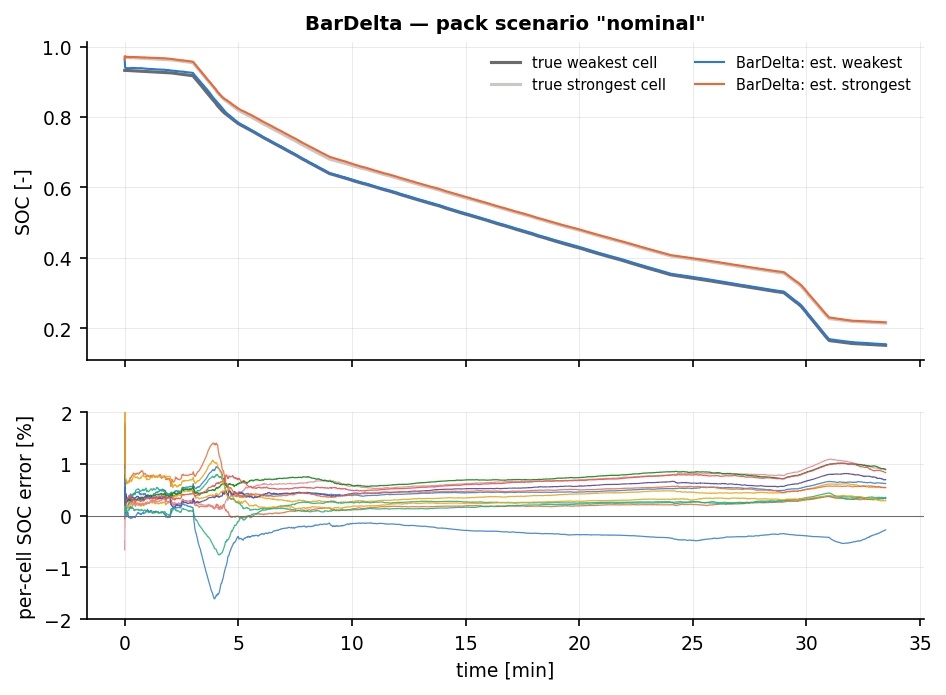
\includegraphics[width=\textwidth]{figures/pack_BarDelta_nominal.png}
\caption{BarDelta on the nominal eVTOL mission: true and estimated per-cell SOC and the
min/mean/max envelope (top), per-cell estimation error (middle), current profile (bottom).}
\end{figure}
\begin{figure}[H]\centering
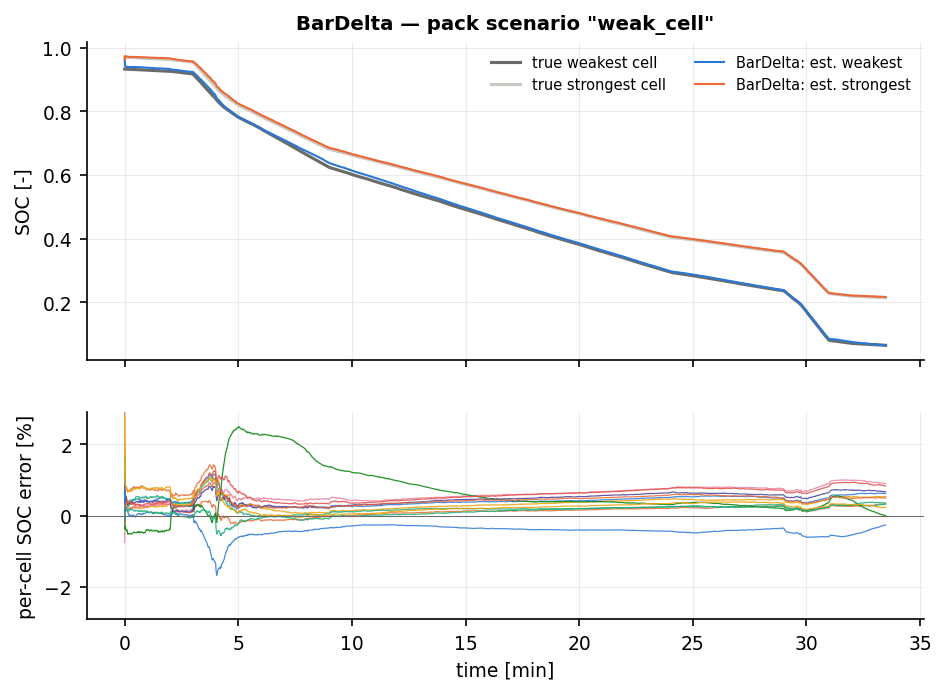
\includegraphics[width=\textwidth]{figures/pack_BarDelta_weak_cell.png}
\caption{BarDelta on \texttt{weak\_cell}: cell 5 has \SI{12}{\percent} less capacity and
\SI{30}{\percent} more resistance than the module average and drifts \num{0.10} SOC below it
over the mission; the delta-capacity state \eqref{eq:bd-deltadyn} follows the ramp.}
\end{figure}

All numbers below are means over three seeds of the eVTOL mission, as printed by
\texttt{bench\_pack --profile evtol --scenario all --seeds 3}. \texttt{rmse\_cells} is the RMS
error over all cells and samples, \texttt{rmse\_min} the RMS error of the reported
weakest-cell SOC (the safety-critical quantity), \texttt{ss} the steady-state value over the
second half of the record and \texttt{max} the worst single-cell error.

\begin{center}\small
\begin{tabular}{@{}lcccc|cccc@{}}
\toprule
& \multicolumn{4}{c|}{\estname{BarDelta}} & \multicolumn{4}{c}{\estname{Decentralized-EKF}} \\
Scenario & rmse & rmse$_{\min}$ & ss & max & rmse & rmse$_{\min}$ & ss & max \\
\midrule
\texttt{nominal}          & 0.0059 & 0.0056 & 0.0065 & 0.031 & 0.0123 & 0.0081 & 0.0134 & 0.046 \\
\texttt{init\_error}      & 0.0064 & 0.0060 & 0.0069 & 0.028 & 0.0118 & 0.0082 & 0.0129 & 0.042 \\
\texttt{current\_bias}    & 0.0084 & 0.0092 & 0.0089 & 0.035 & 0.0137 & 0.0088 & 0.0148 & 0.056 \\
\texttt{weak\_cell}       & 0.0067 & 0.0056 & 0.0070 & 0.030 & 0.0129 & 0.0129 & 0.0137 & 0.048 \\
\texttt{noise\_step}      & 0.0061 & 0.0059 & 0.0067 & 0.031 & 0.0122 & 0.0084 & 0.0131 & 0.045 \\
\texttt{large\_imbalance} & 0.0122 & 0.0218 & 0.0094 & 0.094 & 0.0174 & 0.0245 & 0.0179 & 0.061 \\
\midrule
\si{\nano\second}/step & \multicolumn{4}{c|}{542} & \multicolumn{4}{c}{3860} \\
bytes & \multicolumn{4}{c|}{5616} & \multicolumn{4}{c}{52032} \\
messages/step & \multicolumn{4}{c|}{12} & \multicolumn{4}{c}{0} \\
\bottomrule
\end{tabular}
\end{center}

\paragraph{Computational saving.} $\num{3860}/\num{542} = \num{7.1}\times$ in time and
$\num{52032}/\num{5616} = \num{9.3}\times$ in memory relative to the decentralised baseline, at
\emph{better} accuracy in every scenario --- the factor is close to, but below, the ideal $N_c=12$
because the bar filter itself is one full EKF and the harness measures the whole module on one
core. The price is that the module can no longer be estimated cell-locally: the \num{12} cell
voltages must reach one node every sample (\num{12} numbers per sample, versus \num{0} for the
decentralised baseline). On a daisy-chained cell-monitor bus that traffic already exists for
balancing and safety, so in practice the communication is free.

\paragraph{Why it is more accurate than $N_c$ independent EKFs.} The bar filter sees a
measurement whose sensor noise is $\sqrt{12}$ times smaller than that of any single channel
\eqref{eq:bd-Rbar}, so the common mode --- which carries essentially all of the SOC information
--- is estimated with a bandwidth that no single-cell filter can afford. The decentralised
baseline has to extract the same information twelve times, each time from one noisy channel, and
its steady-state error \num{0.0134} is exactly the single-cell EKF floor.

\paragraph{The delta model earns its states.} Ablations, measured in one paired run over two
seeds so that every variant sees identical data (the default row therefore differs in the last
digit from the three-seed table above); \texttt{nominal} and \texttt{weak\_cell}, rmse and
rmse$_{\min}$:
\begin{center}\small
\begin{tabular}{@{}lcccc@{}}
\toprule
Variant & nom.\ rmse & nom.\ rmse$_{\min}$ & weak rmse & weak rmse$_{\min}$ \\
\midrule
default (3 states, nonlinear OCV)      & 0.0056 & 0.0046 & 0.0060 & 0.0057 \\
no $\Delta q$ state (random-walk $\Delta\soc$)    & 0.0056 & 0.0061 & 0.0073 & 0.0112 \\
no $\Delta\rho$ state                  & 0.0156 & 0.0106 & 0.0176 & 0.0230 \\
tangent OCV in \eqref{eq:bd-deltameas} & 0.0058 & 0.0057 & 0.0086 & 0.0152 \\
multiplicative regressor $w=\bar R_0 i+\bar v_1+\bar v_2$ & 0.0047 & 0.0049 & 0.0068 & 0.0090 \\
no Jensen correction                   & 0.0056 & 0.0042 & 0.0063 & 0.0063 \\
\bottomrule
\end{tabular}
\end{center}
The impedance state is indispensable --- without it the deviation
\eqref{eq:bd-deltameas} is dominated by $\Delta\rho_j w$, which is $\pm\SI{11}{\milli\volt}$ in
cruise against a \SI{2}{\milli\volt} sensor noise, and the filter attributes it to
$\Delta\soc_j$ (nominal rmse triples, worst-cell error \num{0.103}). The capacity state doubles
the weak-cell accuracy (rmse$_{\min}$ \num{0.0057} versus \num{0.0112}), and the exact OCV
difference is what keeps the weak cell from running away at low SOC (worst-cell error \num{0.030}
versus \num{0.071}). The multiplicative regressor is slightly better on \texttt{nominal} but
markedly worse on \texttt{weak\_cell} (rmse$_{\min}$ \num{0.0090} versus \num{0.0057}), because
the benchmark's aged cell scales $R_0$ and $R_1$ but not $R_2$ --- exactly the failure mode that
makes the simple $\Delta R_0$ regressor the safer default.

\paragraph{The reduced rate is free.} In the same paired run, moving the delta filters to
\SI{10}{\hertz} costs \SI{2079}{\nano\second} instead of \SI{536}{\nano\second} per step and buys
$\text{rmse}=\num{0.0054}$ instead of \num{0.0056}; at \SI{0.2}{\hertz} the cost falls to
\SI{399}{\nano\second} with $\text{rmse}=\num{0.0053}$. This is a direct, quantitative
confirmation of Assumption~\ref{as:bd-slow} and of the central engineering claim of
\cite{plett2009bardelta}.

\paragraph{Where it is weakest.} \texttt{large\_imbalance} (initial spread
$\sigma_{\Delta\soc}=\SI{5}{\percent}$, capacity spread \SI{5}{\percent}) is the only scenario in
which the worst single-cell error (\num{0.094}) exceeds that of the decentralised baseline
(\num{0.061}): the transient during which the delta filters learn a \SI{5}{\percent} initial
imbalance from $\pm\SI{35}{\milli\volt}$ of voltage deviation lasts $\sim\SI{100}{\second}$, and
\texttt{max\_cell\_err} records it. The steady-state figure tells the opposite story
(\num{0.0094} versus \num{0.0179}); raising \texttt{delta.sigma\_dz0} to the true spread removes
most of the transient. \texttt{current\_bias} is the hardest scenario for every method here
(\SI{0.25}{\ampere} bias plus \SI{2}{\percent} gain error on a \SI{5}{\ampere\hour} cell): the
bias is a common-mode error of the bar filter that the deviations cannot see, so all four
common-state estimators land within \SI{10}{\percent} of each other at
$\text{rmse}\approx\num{0.008}$.

\section{Summary}
Bar-delta filtering is the method of choice when the number of cells is large, the cells are in
series, and a per-cell SOC must be reported on an embedded budget: it costs one cell filter plus
a negligible per-cell term, it is \num{7}--\num{10} times faster and smaller than one EKF per
cell on this benchmark, and it is more accurate because the common mode is estimated from the
average of $N_c$ voltage channels. Use it with all three delta states --- SOC deviation,
impedance deviation and \emph{capacity} deviation --- otherwise a weak cell is tracked with a
systematic lag, and keep the OCV difference exact once cells can drift more than a few percent
apart. Do not use it when cells are paralleled (the shared-current assumption fails), when a
single module master cannot be given the cell voltages, or when the module-average parameters are
themselves badly wrong: the deviations are blind to a common-mode model error.
